\section{Formulation}\label{sec:game_formulation}

In order to formulate the game theoretic model one needs to define the players
of the game, the strategies of each player and the payoffs of each pair of
strategy being played.

\subsection{Players and parameters}\label{sec:game_players_and_parameters}

The problem studied is a 3-player extensive form game that consists of three
players.
This will later be reduced to a 2-player standard normal form
game~\cite{Maschler2013}.
The three players are:

\begin{itemize}
    \item the decision makers of queueing system \(A\)
    \item the decision makers of queueing system \(B\)
    \item a distribution service that distributes individuals to the two
    queueing systems
\end{itemize}

\begin{figure}[H]
    \centering
    \begin{minipage}{.3\textwidth}
    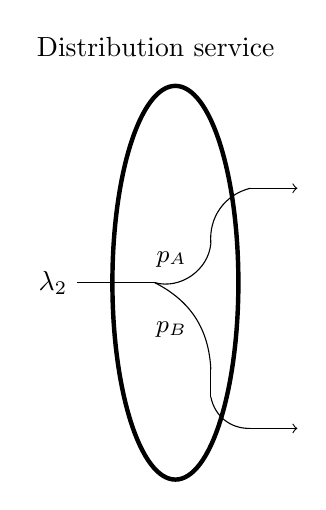
\begin{tikzpicture}
        \draw[ultra thick] (0.75,2) ellipse (0.8cm and 2.5cm);
        \node at (0.5, 5) {Distribution service};
        \draw[-] (0.5, 2) -- ++(-1, 0) node[left] {\(\lambda_2\)};

        % p_A line
        \path (0.49, 2) edge [bend right=50] (1.2, 2.5);
        \path (1.2, 2.5) edge [bend left=40] (1.7, 3.2);
        \draw[->] (1.7, 3.2) -- ++(0.6, 0.);

        % p_B line
        \path (0.49, 2) edge [bend left=30] (1.2, 0.9);
        \draw[-] (1.2, 0.9) -- (1.2, 0.55);
        \path (1.2, 0.55) edge [bend right=40] (1.7, 0.15);
        \draw[->] (1.7, 0.15) -- ++(0.6, 0.);

        \node at (0.7, 2.3) {\small{\( p_A \)}};
        \node at (0.7, 1.4) {\small{\( p_B \)}};
    \end{tikzpicture}
\end{minipage}
\begin{minipage}{.65\textwidth}
    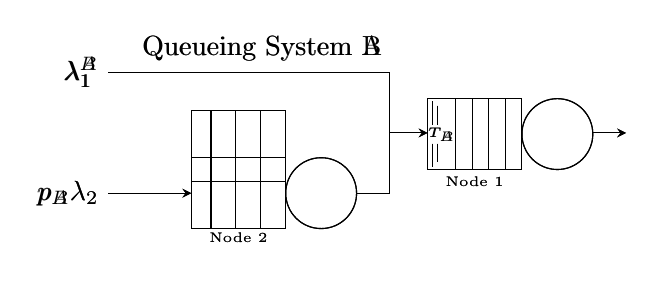
\begin{tikzpicture}[>=stealth, scale=0.6] %arrow type
        % Difference between the two queue diagrams
        
        \tikzmath{
            let \diff = -5cm;
        }
            
        % QUEUEING SYSTEM A

        \node at (1.5cm, 2.3cm) {Queueing System A};
            
        % the rectangle with vertical lines (Node 2)
        \draw (0,0) -- ++(2cm,0) -- ++(0,-1.5cm) -- ++(-2cm,0);
        \foreach \i in {1,...,3, 3.8}
        \draw (2cm-\i*15pt,0) -- +(0,-1.5cm);
        \node at (1, -1.7) {\tiny{Node 2}};

        % the circle (Node 2)
        \draw (2.75,-0.75cm) circle [radius=0.75cm];

        % the rectangle with vertical lines (Node 1)
        \draw (5,1.25) -- ++(2cm,0) -- ++(0,-1.5cm) -- ++(-2cm,0);
        \foreach \i in {1,...,4, 5.7}
        \draw (7cm-\i*10pt,1.25) -- +(0,-1.5cm);
        \node at (6, -0.5) {\tiny{Node 1}};

        % The two vertical lines at the start of Node 1
        \draw (7cm-54pt, 1.2cm) -- +(0,-0.5cm);
        \draw (7cm-54pt, 0.3cm) -- +(0,-0.5cm);
        \draw (7cm-51pt, 1.1cm) -- +(0,-0.4cm);
        \draw (7cm-51pt, 0.3cm) -- +(0,-0.4cm);

        % The label between the lines for T
        \node[anchor=north] at (5.3, 0.84) {\tiny{\( T_A \)}};

        % the circle (Node 1)
        \draw (7.75,0.5) circle [radius=0.75cm];

        % the arrows and labels (Node 2+2)
        \draw[->] (8.5,0.525) -- +(20pt,0);
        \node[align=center] at (1cm,-2cm) {};
        \node[align=center] at (6cm,-0.75cm) {};

        % Ambulance lines
        \draw[<-] (0,-0.75) -- +(-50pt,0) node[left] {\( p_A \lambda_2 \)};
        \draw[-] (3.5,-0.75) -- +(20pt,0);
        \draw (4.2, 0.525) -- (4.2, -0.75);

        % Others lines
        \draw (4.2, 1.8) -- +(-169.5pt,0) node[left] {\( \lambda_1^A \)};
        \draw (4.2, 1.8) -- (4.2, 0.525);
        \draw[->] (4.2, 0.525) -- (5, 0.525);


        % QUEUEING SYSTEM B

        \node at (1.5cm, \diff + 2.3cm) {Queueing System B};

        % the rectangle with vertical rules (Node 2)
        \draw (0, \diff) -- ++(2cm,0) -- ++(0,-1.5cm) -- ++(-2cm,0);
        \foreach \i in {1,...,3, 3.8}
        \draw (2cm-\i*15pt,\diff) -- +(0,-1.5cm);
        \node at (1cm, \diff - 1.7cm) {\tiny{Node 2}};

        % the circle (Node 2)
        \draw (2.75,\diff - 0.75cm) circle [radius=0.75cm];

        % the rectangle with vertical rules (Queue 2)
        \draw (5,\diff + 1.25cm) -- ++(2cm,0) -- ++(0,-1.5cm) -- ++(-2cm,0);
        \foreach \i in {1,...,4, 5.7}
        \draw (7cm-\i*10pt,\diff + 1.25cm) -- +(0,-1.5cm);
        \node at (6, \diff - 0.5cm) {\tiny{Node 1}};

        % The two vertical lines at the start of Queue 2
        \draw (7cm-54pt,\diff + 1.2cm) -- +(0,-0.5cm);
        \draw (7cm-54pt,\diff + 0.3cm) -- +(0,-0.5cm);
        \draw (7cm-51pt,\diff + 1.1cm) -- +(0,-0.4cm);
        \draw (7cm-51pt,\diff + 0.3cm) -- +(0,-0.4cm);

        % The label between the lines for T
        \node[anchor=north] at (5.3, \diff + 0.84cm) {\tiny{\( T_B \)}};

        % the circle (Queue 2)
        \draw (7.75,\diff + 0.5cm) circle [radius=0.75cm];

        % the arrows and labels (Node 2+2)
        \draw[->] (8.5, \diff + 0.525cm) -- +(20pt,0);
        \node[align=center] at (1cm,\diff-2cm) {};
        \node[align=center] at (6cm,\diff-0.75cm) {};

        % Ambulance lines
        \draw[<-] (0, \diff - 0.75cm) -- +(-50pt,0) node[left]
        {\( p_B \lambda_2 \)};
        \draw[-] (3.5, \diff - 0.75cm) -- +(20pt,0);
        \draw (4.2, \diff + 0.525cm) -- (4.2, \diff - 0.75cm);

        % Others lines
        \draw (4.2, \diff + 1.8cm) -- +(-169.5pt,0) node[left]
        {\( \lambda_1^B \)};
        \draw (4.2, \diff + 1.8cm) -- (4.2, \diff + 0.525);
        \draw[->] (4.2, \diff + 0.525cm) -- (5, \diff + 0.525cm);
    \end{tikzpicture}
\end{minipage}

    \caption{A diagrammatic representation of the game theoretic model.
    Individuals arrive at the distribution service at a rate of \( \lambda_2 \)
    and then a proportion of them are distributed to Queueing system \(A\)
    (\(p_A\)) and the remaining proportion to Queueing system \(B\) (\(p_B\))
    so that \(p_A + p_B = 1\).
    The corresponding arrival rates of type 2 individuals to Queueing systems
    \(A\) and \(B\) are thus given by:
    \( p_A \lambda_2 \) and \( p_B \lambda_2 \).}
    \label{fig:diagram_of_game_theoretic_model}
\end{figure}

Each player has their own objective which they aim to optimise.
More specifically, the queueing systems' objective is captured by an upper bound
of the time that a fixed proportion of individuals spend in the system,
while the distribution service aims to minimise the time that its individuals
stay blocked at each queueing system's node 2.
These objectives are more formally defined in Section~\ref{sec:game_strategies}.
The parameters of the game theoretic model are:

\begin{itemize}
    \item \(\lambda_2\): The arrival rate of type 2 individuals arriving at the
    distribution service that need to be distributed to the queueing systems
    \item \(\lambda_{1_i}\): The arrival rate of type 1 individuals to queueing
    system \(i\in\{A, B\}\)
    \item \(\mu_i\): The service rate of individuals at queueing system
    \(i\in\{A, B\}\)
    \item \(C_i\): The number of servers in queueing system \(i\in\{A, B\}\)
    \item \(T_i\): The strategy that queueing system \(i\in\{A, B\} \) chooses
    to play which corresponds to the threshold at which they start blocking
    type 2 individuals at node 2.
    \item \(N_i\): The total capacity of node 1 in queueing system
    \(i\in\{A, B\}\)
    \item \(M_i\): The total capacity of node 2 in queueing system
    \(i\in\{A, B\}\)
    \item \(t\): The time target for both queueing systems
    \item \(\alpha \in [0, 1]\) : Weighted average of blocking time and
    lost individuals (defined in equation~\eqref{eq:obj_distributor_penalty})
\end{itemize}

\subsection{Strategies}\label{sec:game_strategies}

Each player is given a predetermined set of strategies from which to choose.
The strategies of the two queueing systems are the range of thresholds that they
can choose from.
In essence the strategy space of queueing system \(A\) is the set of integers
from
1 to the capacity of node 1 in queueing system \(A\) (\(N_A\)), while the
strategy space of queueing system \(B\) is the set of integers from 1 to the
capacity of node 1 in queueing system \(B\) (\(N_B\)).

\begin{equation}\label{eq:game_strategy_space_queueing_systems}
    T_A \in \{1, 2, \ldots, N_A\} \quad \text{and} \quad
    T_B \in \{1, 2, \ldots, N_B\}
\end{equation}

In essence this means that for either queueing system  (\(A\) or \(B\)), every
strategy
choice generates a different queueing network of the form that is described in
Section~\ref{sec:queueing_section}.
In other words, different strategies are equivalent to different thresholds
which is one of the core parameters of the queueing network.
Consider queueing system \(A\) as one of the three players of the game theoretic
model with node 1 capacity of \(N_A = 6\) and node 2 capacity of \(M_A = 3\).
The strategy space of queueing system \(A\) is then
\(T_A \in \{1, 2, 3, 4, 5, 6\}\).
Every possible value of \(T_A\) corresponds to a different queueing network.
Figures~\ref{fig:game_strategy_visualisation_N_6_M_3_first}
-~\ref{fig:game_strategy_visualisation_N_6_M_3_last} show all possible Markov chain
models that arise from such a strategy space.

\begin{figure}[H]
    \centering
    \scalebox{0.8}{
        \begin{tikzpicture}[-, node distance = 1cm, auto]
\node[state] (u0v0) {(0,0)};
\node[state, right=of u0v0] (u0v1) {(0,1)};
\draw[->](u0v0) edge[bend left] node {\( \Lambda \)} (u0v1);
\draw[->](u0v1) edge[bend left] node {\(\mu \)} (u0v0);
\node[state, below=of u0v1] (u1v1) {(1,1)};
\draw[->](u0v1) edge[bend left] node {\( \lambda_2 \)} (u1v1);
\draw[->](u1v1) edge[bend left] node {\(\mu \)} (u0v1);
\node[state, below=of u1v1] (u2v1) {(2,1)};
\draw[->](u1v1) edge[bend left] node {\( \lambda_2 \)} (u2v1);
\draw[->](u2v1) edge[bend left] node {\(\mu \)} (u1v1);
\node[state, below=of u2v1] (u3v1) {(3,1)};
\draw[->](u2v1) edge[bend left] node {\( \lambda_2 \)} (u3v1);
\draw[->](u3v1) edge[bend left] node {\(\mu \)} (u2v1);
\node[state, right=of u0v1] (u0v2) {(0,2)};
\draw[->](u0v1) edge[bend left] node {\( \lambda_1 \)} (u0v2);
\draw[->](u0v2) edge[bend left] node {\(\mu \)} (u0v1);
\node[state, right=of u1v1] (u1v2) {(1,2)};
\draw[->](u1v1) edge[bend left] node {\( \lambda_1 \)} (u1v2);
\draw[->](u1v2) edge[bend left] node {\(\mu \)} (u1v1);
\draw[->](u0v2) edge node {\( \lambda_2 \)} (u1v2);
\node[state, right=of u2v1] (u2v2) {(2,2)};
\draw[->](u2v1) edge[bend left] node {\( \lambda_1 \)} (u2v2);
\draw[->](u2v2) edge[bend left] node {\(\mu \)} (u2v1);
\draw[->](u1v2) edge node {\( \lambda_2 \)} (u2v2);
\node[state, right=of u3v1] (u3v2) {(3,2)};
\draw[->](u3v1) edge[bend left] node {\( \lambda_1 \)} (u3v2);
\draw[->](u3v2) edge[bend left] node {\(\mu \)} (u3v1);
\draw[->](u2v2) edge node {\( \lambda_2 \)} (u3v2);
\node[state, right=of u0v2] (u0v3) {(0,3)};
\draw[->](u0v2) edge[bend left] node {\( \lambda_1 \)} (u0v3);
\draw[->](u0v3) edge[bend left] node {\(\mu \)} (u0v2);
\node[state, right=of u1v2] (u1v3) {(1,3)};
\draw[->](u1v2) edge[bend left] node {\( \lambda_1 \)} (u1v3);
\draw[->](u1v3) edge[bend left] node {\(\mu \)} (u1v2);
\draw[->](u0v3) edge node {\( \lambda_2 \)} (u1v3);
\node[state, right=of u2v2] (u2v3) {(2,3)};
\draw[->](u2v2) edge[bend left] node {\( \lambda_1 \)} (u2v3);
\draw[->](u2v3) edge[bend left] node {\(\mu \)} (u2v2);
\draw[->](u1v3) edge node {\( \lambda_2 \)} (u2v3);
\node[state, right=of u3v2] (u3v3) {(3,3)};
\draw[->](u3v2) edge[bend left] node {\( \lambda_1 \)} (u3v3);
\draw[->](u3v3) edge[bend left] node {\(\mu \)} (u3v2);
\draw[->](u2v3) edge node {\( \lambda_2 \)} (u3v3);
\node[state, right=of u0v3] (u0v4) {(0,4)};
\draw[->](u0v3) edge[bend left] node {\( \lambda_1 \)} (u0v4);
\draw[->](u0v4) edge[bend left] node {\(\mu \)} (u0v3);
\node[state, right=of u1v3] (u1v4) {(1,4)};
\draw[->](u1v3) edge[bend left] node {\( \lambda_1 \)} (u1v4);
\draw[->](u1v4) edge[bend left] node {\(\mu \)} (u1v3);
\draw[->](u0v4) edge node {\( \lambda_2 \)} (u1v4);
\node[state, right=of u2v3] (u2v4) {(2,4)};
\draw[->](u2v3) edge[bend left] node {\( \lambda_1 \)} (u2v4);
\draw[->](u2v4) edge[bend left] node {\(\mu \)} (u2v3);
\draw[->](u1v4) edge node {\( \lambda_2 \)} (u2v4);
\node[state, right=of u3v3] (u3v4) {(3,4)};
\draw[->](u3v3) edge[bend left] node {\( \lambda_1 \)} (u3v4);
\draw[->](u3v4) edge[bend left] node {\(\mu \)} (u3v3);
\draw[->](u2v4) edge node {\( \lambda_2 \)} (u3v4);
\node[state, right=of u0v4] (u0v5) {(0,5)};
\draw[->](u0v4) edge[bend left] node {\( \lambda_1 \)} (u0v5);
\draw[->](u0v5) edge[bend left] node {\(\mu \)} (u0v4);
\node[state, right=of u1v4] (u1v5) {(1,5)};
\draw[->](u1v4) edge[bend left] node {\( \lambda_1 \)} (u1v5);
\draw[->](u1v5) edge[bend left] node {\(\mu \)} (u1v4);
\draw[->](u0v5) edge node {\( \lambda_2 \)} (u1v5);
\node[state, right=of u2v4] (u2v5) {(2,5)};
\draw[->](u2v4) edge[bend left] node {\( \lambda_1 \)} (u2v5);
\draw[->](u2v5) edge[bend left] node {\(\mu \)} (u2v4);
\draw[->](u1v5) edge node {\( \lambda_2 \)} (u2v5);
\node[state, right=of u3v4] (u3v5) {(3,5)};
\draw[->](u3v4) edge[bend left] node {\( \lambda_1 \)} (u3v5);
\draw[->](u3v5) edge[bend left] node {\(\mu \)} (u3v4);
\draw[->](u2v5) edge node {\( \lambda_2 \)} (u3v5);
\node[state, right=of u0v5] (u0v6) {(0,6)};
\draw[->](u0v5) edge[bend left] node {\( \lambda_1 \)} (u0v6);
\draw[->](u0v6) edge[bend left] node {\(\mu \)} (u0v5);
\node[state, right=of u1v5] (u1v6) {(1,6)};
\draw[->](u1v5) edge[bend left] node {\( \lambda_1 \)} (u1v6);
\draw[->](u1v6) edge[bend left] node {\(\mu \)} (u1v5);
\draw[->](u0v6) edge node {\( \lambda_2 \)} (u1v6);
\node[state, right=of u2v5] (u2v6) {(2,6)};
\draw[->](u2v5) edge[bend left] node {\( \lambda_1 \)} (u2v6);
\draw[->](u2v6) edge[bend left] node {\(\mu \)} (u2v5);
\draw[->](u1v6) edge node {\( \lambda_2 \)} (u2v6);
\node[state, right=of u3v5] (u3v6) {(3,6)};
\draw[->](u3v5) edge[bend left] node {\( \lambda_1 \)} (u3v6);
\draw[->](u3v6) edge[bend left] node {\(\mu \)} (u3v5);
\draw[->](u2v6) edge node {\( \lambda_2 \)} (u3v6);
\end{tikzpicture}
    }
    \caption{\(T_A = 1\)}
    \label{fig:game_strategy_visualisation_N_6_M_3_first}
\end{figure}

\begin{figure}[H]
    \centering
    \scalebox{0.8}{
        \begin{tikzpicture}[-, node distance = 1cm, auto]
\node[state] (u0v0) {(0,0)};
\node[state, right=of u0v0] (u0v1) {(0,1)};
\draw[->](u0v0) edge[bend left] node {\( \Lambda \)} (u0v1);
\draw[->](u0v1) edge[bend left] node {\(\mu \)} (u0v0);
\node[state, right=of u0v1] (u0v2) {(0,2)};
\draw[->](u0v1) edge[bend left] node {\( \Lambda \)} (u0v2);
\draw[->](u0v2) edge[bend left] node {\(\mu \)} (u0v1);
\node[state, below=of u0v2] (u1v2) {(1,2)};
\draw[->](u0v2) edge[bend left] node {\( \lambda_2 \)} (u1v2);
\draw[->](u1v2) edge[bend left] node {\(\mu \)} (u0v2);
\node[state, below=of u1v2] (u2v2) {(2,2)};
\draw[->](u1v2) edge[bend left] node {\( \lambda_2 \)} (u2v2);
\draw[->](u2v2) edge[bend left] node {\(\mu \)} (u1v2);
\node[state, below=of u2v2] (u3v2) {(3,2)};
\draw[->](u2v2) edge[bend left] node {\( \lambda_2 \)} (u3v2);
\draw[->](u3v2) edge[bend left] node {\(\mu \)} (u2v2);
\node[state, right=of u0v2] (u0v3) {(0,3)};
\draw[->](u0v2) edge[bend left] node {\( \lambda_1 \)} (u0v3);
\draw[->](u0v3) edge[bend left] node {\(\mu \)} (u0v2);
\node[state, right=of u1v2] (u1v3) {(1,3)};
\draw[->](u1v2) edge[bend left] node {\( \lambda_1 \)} (u1v3);
\draw[->](u1v3) edge[bend left] node {\(\mu \)} (u1v2);
\draw[->](u0v3) edge node {\( \lambda_2 \)} (u1v3);
\node[state, right=of u2v2] (u2v3) {(2,3)};
\draw[->](u2v2) edge[bend left] node {\( \lambda_1 \)} (u2v3);
\draw[->](u2v3) edge[bend left] node {\(\mu \)} (u2v2);
\draw[->](u1v3) edge node {\( \lambda_2 \)} (u2v3);
\node[state, right=of u3v2] (u3v3) {(3,3)};
\draw[->](u3v2) edge[bend left] node {\( \lambda_1 \)} (u3v3);
\draw[->](u3v3) edge[bend left] node {\(\mu \)} (u3v2);
\draw[->](u2v3) edge node {\( \lambda_2 \)} (u3v3);
\node[state, right=of u0v3] (u0v4) {(0,4)};
\draw[->](u0v3) edge[bend left] node {\( \lambda_1 \)} (u0v4);
\draw[->](u0v4) edge[bend left] node {\(\mu \)} (u0v3);
\node[state, right=of u1v3] (u1v4) {(1,4)};
\draw[->](u1v3) edge[bend left] node {\( \lambda_1 \)} (u1v4);
\draw[->](u1v4) edge[bend left] node {\(\mu \)} (u1v3);
\draw[->](u0v4) edge node {\( \lambda_2 \)} (u1v4);
\node[state, right=of u2v3] (u2v4) {(2,4)};
\draw[->](u2v3) edge[bend left] node {\( \lambda_1 \)} (u2v4);
\draw[->](u2v4) edge[bend left] node {\(\mu \)} (u2v3);
\draw[->](u1v4) edge node {\( \lambda_2 \)} (u2v4);
\node[state, right=of u3v3] (u3v4) {(3,4)};
\draw[->](u3v3) edge[bend left] node {\( \lambda_1 \)} (u3v4);
\draw[->](u3v4) edge[bend left] node {\(\mu \)} (u3v3);
\draw[->](u2v4) edge node {\( \lambda_2 \)} (u3v4);
\node[state, right=of u0v4] (u0v5) {(0,5)};
\draw[->](u0v4) edge[bend left] node {\( \lambda_1 \)} (u0v5);
\draw[->](u0v5) edge[bend left] node {\(\mu \)} (u0v4);
\node[state, right=of u1v4] (u1v5) {(1,5)};
\draw[->](u1v4) edge[bend left] node {\( \lambda_1 \)} (u1v5);
\draw[->](u1v5) edge[bend left] node {\(\mu \)} (u1v4);
\draw[->](u0v5) edge node {\( \lambda_2 \)} (u1v5);
\node[state, right=of u2v4] (u2v5) {(2,5)};
\draw[->](u2v4) edge[bend left] node {\( \lambda_1 \)} (u2v5);
\draw[->](u2v5) edge[bend left] node {\(\mu \)} (u2v4);
\draw[->](u1v5) edge node {\( \lambda_2 \)} (u2v5);
\node[state, right=of u3v4] (u3v5) {(3,5)};
\draw[->](u3v4) edge[bend left] node {\( \lambda_1 \)} (u3v5);
\draw[->](u3v5) edge[bend left] node {\(\mu \)} (u3v4);
\draw[->](u2v5) edge node {\( \lambda_2 \)} (u3v5);
\node[state, right=of u0v5] (u0v6) {(0,6)};
\draw[->](u0v5) edge[bend left] node {\( \lambda_1 \)} (u0v6);
\draw[->](u0v6) edge[bend left] node {\(\mu \)} (u0v5);
\node[state, right=of u1v5] (u1v6) {(1,6)};
\draw[->](u1v5) edge[bend left] node {\( \lambda_1 \)} (u1v6);
\draw[->](u1v6) edge[bend left] node {\(\mu \)} (u1v5);
\draw[->](u0v6) edge node {\( \lambda_2 \)} (u1v6);
\node[state, right=of u2v5] (u2v6) {(2,6)};
\draw[->](u2v5) edge[bend left] node {\( \lambda_1 \)} (u2v6);
\draw[->](u2v6) edge[bend left] node {\(\mu \)} (u2v5);
\draw[->](u1v6) edge node {\( \lambda_2 \)} (u2v6);
\node[state, right=of u3v5] (u3v6) {(3,6)};
\draw[->](u3v5) edge[bend left] node {\( \lambda_1 \)} (u3v6);
\draw[->](u3v6) edge[bend left] node {\(\mu \)} (u3v5);
\draw[->](u2v6) edge node {\( \lambda_2 \)} (u3v6);
\end{tikzpicture}
    }
    \caption{\(T_A = 2\)}
\end{figure}

\begin{figure}[H]
    \centering
    \scalebox{0.8}{
        \begin{tikzpicture}[-, node distance = 1cm, auto]
\node[state] (u0v0) {(0,0)};
\node[state, right=of u0v0] (u0v1) {(0,1)};
\draw[->](u0v0) edge[bend left] node {\( \Lambda \)} (u0v1);
\draw[->](u0v1) edge[bend left] node {\(\mu \)} (u0v0);
\node[state, right=of u0v1] (u0v2) {(0,2)};
\draw[->](u0v1) edge[bend left] node {\( \Lambda \)} (u0v2);
\draw[->](u0v2) edge[bend left] node {\(\mu \)} (u0v1);
\node[state, right=of u0v2] (u0v3) {(0,3)};
\draw[->](u0v2) edge[bend left] node {\( \Lambda \)} (u0v3);
\draw[->](u0v3) edge[bend left] node {\(\mu \)} (u0v2);
\node[state, below=of u0v3] (u1v3) {(1,3)};
\draw[->](u0v3) edge[bend left] node {\( \lambda_2 \)} (u1v3);
\draw[->](u1v3) edge[bend left] node {\(\mu \)} (u0v3);
\node[state, below=of u1v3] (u2v3) {(2,3)};
\draw[->](u1v3) edge[bend left] node {\( \lambda_2 \)} (u2v3);
\draw[->](u2v3) edge[bend left] node {\(\mu \)} (u1v3);
\node[state, below=of u2v3] (u3v3) {(3,3)};
\draw[->](u2v3) edge[bend left] node {\( \lambda_2 \)} (u3v3);
\draw[->](u3v3) edge[bend left] node {\(\mu \)} (u2v3);
\node[state, right=of u0v3] (u0v4) {(0,4)};
\draw[->](u0v3) edge[bend left] node {\( \lambda_1 \)} (u0v4);
\draw[->](u0v4) edge[bend left] node {\(\mu \)} (u0v3);
\node[state, right=of u1v3] (u1v4) {(1,4)};
\draw[->](u1v3) edge[bend left] node {\( \lambda_1 \)} (u1v4);
\draw[->](u1v4) edge[bend left] node {\(\mu \)} (u1v3);
\draw[->](u0v4) edge node {\( \lambda_2 \)} (u1v4);
\node[state, right=of u2v3] (u2v4) {(2,4)};
\draw[->](u2v3) edge[bend left] node {\( \lambda_1 \)} (u2v4);
\draw[->](u2v4) edge[bend left] node {\(\mu \)} (u2v3);
\draw[->](u1v4) edge node {\( \lambda_2 \)} (u2v4);
\node[state, right=of u3v3] (u3v4) {(3,4)};
\draw[->](u3v3) edge[bend left] node {\( \lambda_1 \)} (u3v4);
\draw[->](u3v4) edge[bend left] node {\(\mu \)} (u3v3);
\draw[->](u2v4) edge node {\( \lambda_2 \)} (u3v4);
\node[state, right=of u0v4] (u0v5) {(0,5)};
\draw[->](u0v4) edge[bend left] node {\( \lambda_1 \)} (u0v5);
\draw[->](u0v5) edge[bend left] node {\(\mu \)} (u0v4);
\node[state, right=of u1v4] (u1v5) {(1,5)};
\draw[->](u1v4) edge[bend left] node {\( \lambda_1 \)} (u1v5);
\draw[->](u1v5) edge[bend left] node {\(\mu \)} (u1v4);
\draw[->](u0v5) edge node {\( \lambda_2 \)} (u1v5);
\node[state, right=of u2v4] (u2v5) {(2,5)};
\draw[->](u2v4) edge[bend left] node {\( \lambda_1 \)} (u2v5);
\draw[->](u2v5) edge[bend left] node {\(\mu \)} (u2v4);
\draw[->](u1v5) edge node {\( \lambda_2 \)} (u2v5);
\node[state, right=of u3v4] (u3v5) {(3,5)};
\draw[->](u3v4) edge[bend left] node {\( \lambda_1 \)} (u3v5);
\draw[->](u3v5) edge[bend left] node {\(\mu \)} (u3v4);
\draw[->](u2v5) edge node {\( \lambda_2 \)} (u3v5);
\node[state, right=of u0v5] (u0v6) {(0,6)};
\draw[->](u0v5) edge[bend left] node {\( \lambda_1 \)} (u0v6);
\draw[->](u0v6) edge[bend left] node {\(\mu \)} (u0v5);
\node[state, right=of u1v5] (u1v6) {(1,6)};
\draw[->](u1v5) edge[bend left] node {\( \lambda_1 \)} (u1v6);
\draw[->](u1v6) edge[bend left] node {\(\mu \)} (u1v5);
\draw[->](u0v6) edge node {\( \lambda_2 \)} (u1v6);
\node[state, right=of u2v5] (u2v6) {(2,6)};
\draw[->](u2v5) edge[bend left] node {\( \lambda_1 \)} (u2v6);
\draw[->](u2v6) edge[bend left] node {\(\mu \)} (u2v5);
\draw[->](u1v6) edge node {\( \lambda_2 \)} (u2v6);
\node[state, right=of u3v5] (u3v6) {(3,6)};
\draw[->](u3v5) edge[bend left] node {\( \lambda_1 \)} (u3v6);
\draw[->](u3v6) edge[bend left] node {\(\mu \)} (u3v5);
\draw[->](u2v6) edge node {\( \lambda_2 \)} (u3v6);
\end{tikzpicture}
    }
    \caption{\(T_A = 3\)}
\end{figure}


\begin{figure}[H]
    \centering
    \scalebox{0.8}{
        \begin{tikzpicture}[-, node distance = 1cm, auto]
\node[state] (u0v0) {(0,0)};
\node[state, right=of u0v0] (u0v1) {(0,1)};
\draw[->](u0v0) edge[bend left] node {\( \Lambda \)} (u0v1);
\draw[->](u0v1) edge[bend left] node {\(\mu \)} (u0v0);
\node[state, right=of u0v1] (u0v2) {(0,2)};
\draw[->](u0v1) edge[bend left] node {\( \Lambda \)} (u0v2);
\draw[->](u0v2) edge[bend left] node {\(\mu \)} (u0v1);
\node[state, right=of u0v2] (u0v3) {(0,3)};
\draw[->](u0v2) edge[bend left] node {\( \Lambda \)} (u0v3);
\draw[->](u0v3) edge[bend left] node {\(\mu \)} (u0v2);
\node[state, right=of u0v3] (u0v4) {(0,4)};
\draw[->](u0v3) edge[bend left] node {\( \Lambda \)} (u0v4);
\draw[->](u0v4) edge[bend left] node {\(\mu \)} (u0v3);
\node[state, below=of u0v4] (u1v4) {(1,4)};
\draw[->](u0v4) edge[bend left] node {\( \lambda_2 \)} (u1v4);
\draw[->](u1v4) edge[bend left] node {\(\mu \)} (u0v4);
\node[state, below=of u1v4] (u2v4) {(2,4)};
\draw[->](u1v4) edge[bend left] node {\( \lambda_2 \)} (u2v4);
\draw[->](u2v4) edge[bend left] node {\(\mu \)} (u1v4);
\node[state, below=of u2v4] (u3v4) {(3,4)};
\draw[->](u2v4) edge[bend left] node {\( \lambda_2 \)} (u3v4);
\draw[->](u3v4) edge[bend left] node {\(\mu \)} (u2v4);
\node[state, right=of u0v4] (u0v5) {(0,5)};
\draw[->](u0v4) edge[bend left] node {\( \lambda_1 \)} (u0v5);
\draw[->](u0v5) edge[bend left] node {\(\mu \)} (u0v4);
\node[state, right=of u1v4] (u1v5) {(1,5)};
\draw[->](u1v4) edge[bend left] node {\( \lambda_1 \)} (u1v5);
\draw[->](u1v5) edge[bend left] node {\(\mu \)} (u1v4);
\draw[->](u0v5) edge node {\( \lambda_2 \)} (u1v5);
\node[state, right=of u2v4] (u2v5) {(2,5)};
\draw[->](u2v4) edge[bend left] node {\( \lambda_1 \)} (u2v5);
\draw[->](u2v5) edge[bend left] node {\(\mu \)} (u2v4);
\draw[->](u1v5) edge node {\( \lambda_2 \)} (u2v5);
\node[state, right=of u3v4] (u3v5) {(3,5)};
\draw[->](u3v4) edge[bend left] node {\( \lambda_1 \)} (u3v5);
\draw[->](u3v5) edge[bend left] node {\(\mu \)} (u3v4);
\draw[->](u2v5) edge node {\( \lambda_2 \)} (u3v5);
\node[state, right=of u0v5] (u0v6) {(0,6)};
\draw[->](u0v5) edge[bend left] node {\( \lambda_1 \)} (u0v6);
\draw[->](u0v6) edge[bend left] node {\(\mu \)} (u0v5);
\node[state, right=of u1v5] (u1v6) {(1,6)};
\draw[->](u1v5) edge[bend left] node {\( \lambda_1 \)} (u1v6);
\draw[->](u1v6) edge[bend left] node {\(\mu \)} (u1v5);
\draw[->](u0v6) edge node {\( \lambda_2 \)} (u1v6);
\node[state, right=of u2v5] (u2v6) {(2,6)};
\draw[->](u2v5) edge[bend left] node {\( \lambda_1 \)} (u2v6);
\draw[->](u2v6) edge[bend left] node {\(\mu \)} (u2v5);
\draw[->](u1v6) edge node {\( \lambda_2 \)} (u2v6);
\node[state, right=of u3v5] (u3v6) {(3,6)};
\draw[->](u3v5) edge[bend left] node {\( \lambda_1 \)} (u3v6);
\draw[->](u3v6) edge[bend left] node {\(\mu \)} (u3v5);
\draw[->](u2v6) edge node {\( \lambda_2 \)} (u3v6);
\end{tikzpicture}
    }
    \caption{\(T_A = 4\)}
\end{figure}

\begin{figure}[H]
    \centering
    \scalebox{0.8}{
        \begin{tikzpicture}[-, node distance = 1cm, auto]
\node[state] (u0v0) {(0,0)};
\node[state, right=of u0v0] (u0v1) {(0,1)};
\draw[->](u0v0) edge[bend left] node {\( \Lambda \)} (u0v1);
\draw[->](u0v1) edge[bend left] node {\(\mu \)} (u0v0);
\node[state, right=of u0v1] (u0v2) {(0,2)};
\draw[->](u0v1) edge[bend left] node {\( \Lambda \)} (u0v2);
\draw[->](u0v2) edge[bend left] node {\(\mu \)} (u0v1);
\node[state, right=of u0v2] (u0v3) {(0,3)};
\draw[->](u0v2) edge[bend left] node {\( \Lambda \)} (u0v3);
\draw[->](u0v3) edge[bend left] node {\(\mu \)} (u0v2);
\node[state, right=of u0v3] (u0v4) {(0,4)};
\draw[->](u0v3) edge[bend left] node {\( \Lambda \)} (u0v4);
\draw[->](u0v4) edge[bend left] node {\(\mu \)} (u0v3);
\node[state, right=of u0v4] (u0v5) {(0,5)};
\draw[->](u0v4) edge[bend left] node {\( \Lambda \)} (u0v5);
\draw[->](u0v5) edge[bend left] node {\(\mu \)} (u0v4);
\node[state, below=of u0v5] (u1v5) {(1,5)};
\draw[->](u0v5) edge[bend left] node {\( \lambda_2 \)} (u1v5);
\draw[->](u1v5) edge[bend left] node {\(\mu \)} (u0v5);
\node[state, below=of u1v5] (u2v5) {(2,5)};
\draw[->](u1v5) edge[bend left] node {\( \lambda_2 \)} (u2v5);
\draw[->](u2v5) edge[bend left] node {\(\mu \)} (u1v5);
\node[state, below=of u2v5] (u3v5) {(3,5)};
\draw[->](u2v5) edge[bend left] node {\( \lambda_2 \)} (u3v5);
\draw[->](u3v5) edge[bend left] node {\(\mu \)} (u2v5);
\node[state, right=of u0v5] (u0v6) {(0,6)};
\draw[->](u0v5) edge[bend left] node {\( \lambda_1 \)} (u0v6);
\draw[->](u0v6) edge[bend left] node {\(\mu \)} (u0v5);
\node[state, right=of u1v5] (u1v6) {(1,6)};
\draw[->](u1v5) edge[bend left] node {\( \lambda_1 \)} (u1v6);
\draw[->](u1v6) edge[bend left] node {\(\mu \)} (u1v5);
\draw[->](u0v6) edge node {\( \lambda_2 \)} (u1v6);
\node[state, right=of u2v5] (u2v6) {(2,6)};
\draw[->](u2v5) edge[bend left] node {\( \lambda_1 \)} (u2v6);
\draw[->](u2v6) edge[bend left] node {\(\mu \)} (u2v5);
\draw[->](u1v6) edge node {\( \lambda_2 \)} (u2v6);
\node[state, right=of u3v5] (u3v6) {(3,6)};
\draw[->](u3v5) edge[bend left] node {\( \lambda_1 \)} (u3v6);
\draw[->](u3v6) edge[bend left] node {\(\mu \)} (u3v5);
\draw[->](u2v6) edge node {\( \lambda_2 \)} (u3v6);
\end{tikzpicture}
    }
    \caption{\(T_A = 5\)}
\end{figure}

\begin{figure}[H]
    \centering
    \scalebox{0.8}{
        \begin{tikzpicture}[-, node distance = 1cm, auto]
\node[state] (u0v0) {(0,0)};
\node[state, right=of u0v0] (u0v1) {(0,1)};
\draw[->](u0v0) edge[bend left] node {\( \Lambda \)} (u0v1);
\draw[->](u0v1) edge[bend left] node {\(\mu \)} (u0v0);
\node[state, right=of u0v1] (u0v2) {(0,2)};
\draw[->](u0v1) edge[bend left] node {\( \Lambda \)} (u0v2);
\draw[->](u0v2) edge[bend left] node {\(\mu \)} (u0v1);
\node[state, right=of u0v2] (u0v3) {(0,3)};
\draw[->](u0v2) edge[bend left] node {\( \Lambda \)} (u0v3);
\draw[->](u0v3) edge[bend left] node {\(\mu \)} (u0v2);
\node[state, right=of u0v3] (u0v4) {(0,4)};
\draw[->](u0v3) edge[bend left] node {\( \Lambda \)} (u0v4);
\draw[->](u0v4) edge[bend left] node {\(\mu \)} (u0v3);
\node[state, right=of u0v4] (u0v5) {(0,5)};
\draw[->](u0v4) edge[bend left] node {\( \Lambda \)} (u0v5);
\draw[->](u0v5) edge[bend left] node {\(\mu \)} (u0v4);
\node[state, right=of u0v5] (u0v6) {(0,6)};
\draw[->](u0v5) edge[bend left] node {\( \Lambda \)} (u0v6);
\draw[->](u0v6) edge[bend left] node {\(\mu \)} (u0v5);
\node[state, below=of u0v6] (u1v6) {(1,6)};
\draw[->](u0v6) edge[bend left] node {\( \lambda_2 \)} (u1v6);
\draw[->](u1v6) edge[bend left] node {\(\mu \)} (u0v6);
\node[state, below=of u1v6] (u2v6) {(2,6)};
\draw[->](u1v6) edge[bend left] node {\( \lambda_2 \)} (u2v6);
\draw[->](u2v6) edge[bend left] node {\(\mu \)} (u1v6);
\node[state, below=of u2v6] (u3v6) {(3,6)};
\draw[->](u2v6) edge[bend left] node {\( \lambda_2 \)} (u3v6);
\draw[->](u3v6) edge[bend left] node {\(\mu \)} (u2v6);
\end{tikzpicture}
    }
    \caption{\(T_A = 6\)}
    \label{fig:game_strategy_visualisation_N_6_M_3_last}
\end{figure}

Each of these Markov chains generate unique performance measures, state
probabilities and overall queueing network behaviour.
By varying the threshold \(T_A\) from 1 to 6, the queueing network of queueing
system \(A\) has a significant change in the mean waiting time and in the mean
blocking time.
As a matter of fact, as the threshold is increased the mean waiting time is
non-increasing while the mean blocking time is non-decreasing.
Having a low threshold means that queueing system \(A\) will block type 2
individuals more often and thus the mean blocking time will be higher and
hence the mean waiting time will be lower.
The same logic applies to queueing system \(B\).

The strategy space of the distribution service, which is the third player of the
game is the range of all possible ways to distribute individuals to the two
queueing systems.
That is the proportions of individuals to send to queueing system \(A\) and the
proportion of individuals to send to queueing system \(B\) (\(p_A, p_B\)).

\begin{align}
    p_A \in & [0, 1] \quad \text{and} \quad p_B \in [0, 1] \nonumber \\
    \text{such that} & \quad p_A + p_B = 1, p_A, p_B > 0
    \label{eq:game_strategy_space_distribution_service_full}
\end{align}

Since \(p_B\) is dependent on \(p_A\) and vice versa,
equation~\eqref{eq:game_strategy_space_distribution_service_full} can be further
simplified so that the strategy space is defined solely by \(p_A\).

\begin{equation}\label{eq:game_strategy_space_distribution_service_simplified}
    p_A \in [0, 1] \quad \text{and} \quad p_B = 1 - p_A
\end{equation}

Similar to the strategy space of the queueing networks, the strategy space of
the distribution service is also translated back into the queueing network.
Different values of \(p_A\) and \(p_B\), directly affect the arrival rates of
type 2 individuals to the two queueing systems.
In fact the arrival rate of type 2 individuals to queueing system \(A\) is
\(p_A \lambda_2\) and to queueing system \(B\) is \(p_B \lambda_2\).
Thus by increasing \(p_A\) both the mean waiting time and the mean blocking time
of queueing system \(A\) will increase but equivalently will decrease for
queueing system \(B\).


\subsection{Payoffs}

Consider the three players of the game; queueing system \(A\), queueing system
\(B\) and
the distribution service.
Apart from a strategy space each player also has some objective that they would
want to either minimise or maximise.

\begin{figure}[H]
    \begin{minipage}{.3\textwidth}
    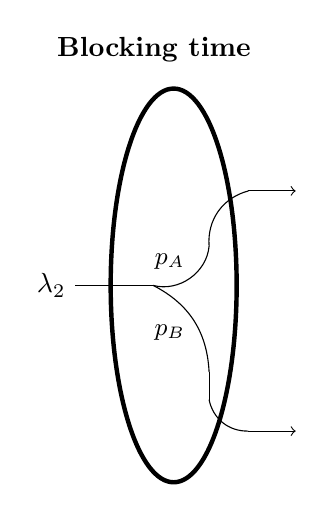
\begin{tikzpicture}
        \draw[ultra thick] (0.75,2) ellipse (0.8cm and 2.5cm);
        \node at (0.5, 5) {\textbf{Blocking time}};
        \draw[-] (0.5, 2) -- ++(-1, 0) node[left] {\(\lambda_2\)};

        % p_A line
        \path (0.49, 2) edge [bend right=50] (1.2, 2.5);
        \path (1.2, 2.5) edge [bend left=40] (1.7, 3.2);
        \draw[->] (1.7, 3.2) -- ++(0.6, 0.);

        % p_B line
        \path (0.49, 2) edge [bend left=30] (1.2, 0.9);
        \draw[-] (1.2, 0.9) -- (1.2, 0.55);
        \path (1.2, 0.55) edge [bend right=40] (1.7, 0.15);
        \draw[->] (1.7, 0.15) -- ++(0.6, 0.);

        \node at (0.7, 2.3) {\small{\( p_A \)}};
        \node at (0.7, 1.4) {\small{\( p_B \)}};
    \end{tikzpicture}
\end{minipage}
\begin{minipage}{.65\textwidth}
    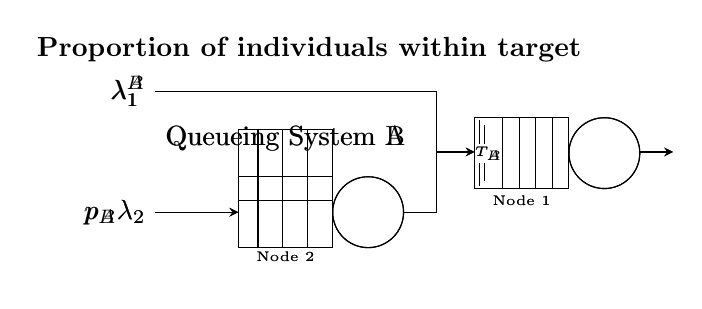
\begin{tikzpicture}[>=stealth, scale=0.6] %arrow type
        % Difference between the two queue diagrams
        
        \tikzmath{
            let \diff = -5cm;
        }
            
        % QUEUEING SYSTEM A
        \node at (1.5cm, 2.7cm) {\textbf{Proportion of individuals within target}};
        \node at (1cm, 0.8cm) {Queueing System A};
            
        % the rectangle with vertical lines (Node 2)
        \draw (0,0) -- ++(2cm,0) -- ++(0,-1.5cm) -- ++(-2cm,0);
        \foreach \i in {1,...,3, 3.8}
        \draw (2cm-\i*15pt,0) -- +(0,-1.5cm);
        \node at (1, -1.7) {\tiny{Node 2}};

        % the circle (Node 2)
        \draw (2.75,-0.75cm) circle [radius=0.75cm];

        % the rectangle with vertical lines (Node 1)
        \draw (5,1.25) -- ++(2cm,0) -- ++(0,-1.5cm) -- ++(-2cm,0);
        \foreach \i in {1,...,4, 5.7}
        \draw (7cm-\i*10pt,1.25) -- +(0,-1.5cm);
        \node at (6, -0.5) {\tiny{Node 1}};

        % The two vertical lines at the start of Node 1
        \draw (7cm-54pt, 1.2cm) -- +(0,-0.5cm);
        \draw (7cm-54pt, 0.3cm) -- +(0,-0.5cm);
        \draw (7cm-51pt, 1.1cm) -- +(0,-0.4cm);
        \draw (7cm-51pt, 0.3cm) -- +(0,-0.4cm);

        % The label between the lines for T
        \node[anchor=north] at (5.3, 0.84) {\tiny{\( T_A \)}};

        % the circle (Node 1)
        \draw (7.75,0.5) circle [radius=0.75cm];

        % the arrows and labels (Node 2+2)
        \draw[->] (8.5,0.525) -- +(20pt,0);
        \node[align=center] at (1cm,-2cm) {};
        \node[align=center] at (6cm,-0.75cm) {};

        % Ambulance lines
        \draw[<-] (0,-0.75) -- +(-50pt,0) node[left] {\( p_A \lambda_2 \)};
        \draw[-] (3.5,-0.75) -- +(20pt,0);
        \draw (4.2, 0.525) -- (4.2, -0.75);

        % Others lines
        \draw (4.2, 1.8) -- +(-169.5pt,0) node[left] {\( \lambda_1^A \)};
        \draw (4.2, 1.8) -- (4.2, 0.525);
        \draw[->] (4.2, 0.525) -- (5, 0.525);


        % QUEUEING SYSTEM B
        \node at (1cm, \diff + 0.8cm) {Queueing System B};

        % the rectangle with vertical rules (Node 2)
        \draw (0, \diff) -- ++(2cm,0) -- ++(0,-1.5cm) -- ++(-2cm,0);
        \foreach \i in {1,...,3, 3.8}
        \draw (2cm-\i*15pt,\diff) -- +(0,-1.5cm);
        \node at (1cm, \diff - 1.7cm) {\tiny{Node 2}};

        % the circle (Node 2)
        \draw (2.75,\diff - 0.75cm) circle [radius=0.75cm];

        % the rectangle with vertical rules (Queue 2)
        \draw (5,\diff + 1.25cm) -- ++(2cm,0) -- ++(0,-1.5cm) -- ++(-2cm,0);
        \foreach \i in {1,...,4, 5.7}
        \draw (7cm-\i*10pt,\diff + 1.25cm) -- +(0,-1.5cm);
        \node at (6, \diff - 0.5cm) {\tiny{Node 1}};

        % The two vertical lines at the start of Queue 2
        \draw (7cm-54pt,\diff + 1.2cm) -- +(0,-0.5cm);
        \draw (7cm-54pt,\diff + 0.3cm) -- +(0,-0.5cm);
        \draw (7cm-51pt,\diff + 1.1cm) -- +(0,-0.4cm);
        \draw (7cm-51pt,\diff + 0.3cm) -- +(0,-0.4cm);

        % The label between the lines for T
        \node[anchor=north] at (5.3, \diff + 0.84cm) {\tiny{\( T_B \)}};

        % the circle (Queue 2)
        \draw (7.75,\diff + 0.5cm) circle [radius=0.75cm];

        % the arrows and labels (Node 2+2)
        \draw[->] (8.5, \diff + 0.525cm) -- +(20pt,0);
        \node[align=center] at (1cm,\diff-2cm) {};
        \node[align=center] at (6cm,\diff-0.75cm) {};

        % Ambulance lines
        \draw[<-] (0, \diff - 0.75cm) -- +(-50pt,0) node[left]
        {\( p_B \lambda_2 \)};
        \draw[-] (3.5, \diff - 0.75cm) -- +(20pt,0);
        \draw (4.2, \diff + 0.525cm) -- (4.2, \diff - 0.75cm);

        % Others lines
        \draw (4.2, \diff + 1.8cm) -- +(-169.5pt,0) node[left]
        {\( \lambda_1^B \)};
        \draw (4.2, \diff + 1.8cm) -- (4.2, \diff + 0.525);
        \draw[->] (4.2, \diff + 0.525cm) -- (5, \diff + 0.525cm);
    \end{tikzpicture}
\end{minipage}

    \caption{A diagrammatic representation of the game theoretic model as shown
    in Figure~\ref{fig:diagram_of_game_theoretic_model} listing the performance
    measures that correspond to each player's utilities.}
    \label{fig:diagram_of_game_theoretic_model_objectives}
\end{figure}


The payoffs of the players are directly related to the performance measures of
the queueing networks.
More specifically the utilities of the queueing systems focus on the proportion
of individuals whose waiting time and service time falls within a predefined
time target, where this is defined in
Section~\ref{sec:proportion_of_individuals_within_time}.
Similarly the utilities of the distribution service focus on the blocking time
of the queueing systems defined in Section~\ref{sec:blocking_time}.

Consider the queueing system players first.
The objective of either queueing system should be to pick a threshold so that
their own mean waiting time is minimised.

\begin{equation}\label{eq:game_theoretic_alternative_objective_queueing_system_A}
    \arg \min_{T_i} \quad \mathbb{E}[W_i] \quad i \in {A, B}
\end{equation}

The mean waiting time is defined in Section~\ref{sec:waiting_time} as the
average time that an individual spends in node 1.
Although this might seem like a sensible objective at first glance, it is not
necessarily a realistic one.
By using the utility function of
equation~\eqref{eq:game_theoretic_alternative_objective_queueing_system_A}
the queueing systems best response will always be to pick strategy of \(T=1\).
A threshold of \(T=1\) will always result in the lowest mean waiting time
since it will prevent type 2 individuals from entering node 1 as long as there
is at least one individual in node 1.
Depending on the number of available servers this might be true for other values
of \(T\) as well.
For example if there is one available server in node 1, then a threshold of
\(T=1\) will always result in a mean waiting time of zero for type 2
individuals.
That is because type 2 individuals can only enter node 1 if there is nobody
else in node 1, which means that there will always be a free server for type 2
individuals.
Similarly if there are two available servers in node 1, then a threshold of
either \(T=1\) or \(T=2\) will also result in a mean waiting time of zero for
type 2 individuals.

Therefore a more sophisticated objective that doesn't force the queueing systems
to pick the lowest threshold is also considered.
The new objective function is defined as:

\begin{equation}\label{eq:obj_queueing_systems}
    \arg \max_{T_i} \quad 1 - \left( \hat{P} - P(W_i < t) \right)^2
    \qquad i \in {A, B}
\end{equation}

where \(W\) is the waiting time of a potential individual, \(t\) is the time
target and \(\hat{P}\) is the percentage target of individuals that need to be
within that target.
In other words, their aim is to find the threshold that minimises the
difference between the probability \(P(W_i < t)\) and the percentage goal,
or maximise its negation.

The third player, the distribution service, has its own choices to make and
its own goals to satisfy.
The strategy set of the third player is a proportion \(0 \leq p_A \leq 1\)
that corresponds to the proportion of individuals to send to queueing system A
(defined in
equation~\eqref{eq:game_strategy_space_distribution_service_simplified}).
The choice of \(p_A\) and \(p_B\), are based on minimising any potential
blockages that may occur, given the pair of thresholds chosen by the two
queueing systems.
Thus, its objective is to minimise the blocked time of the individuals
(\(B_A\) and \(B_B\)) that they send to queueing systems \(A\) and \(B\).

Apart from the time being blocked, an additional aspect that may affect the
decision of the distribution service is the probability that an individual
becomes lost to a queueing system.
A type 2 individual can become lost to a queueing system if they arrive in a
queueing system and node 2 is at its maximum capacity \(M\).
Therefore, the probability that an individual is lost to queueing system \(i\)
is given by \(L_i\) where \(i \in \{A, B\}\):

\begin{equation}\label{eq:probability_lost}
    L_i = \sum_{\substack{(u, v) \in S \\ u = M}} \pi_{(u, v)}
\end{equation}

where \(S\) is the set of all states in queueing system \(i\), \(M\) is the
maximum capacity of node 2 and \(\pi_{(u, v)}\) is the probability of being in
state \((u, v)\) (as defined in Section~\ref{sec:queueing_section}).

For each queueing system, there is a penalty of sending a proportion of \(p_i\)
individuals to that queueing system.
That penalty is given by:

\begin{equation}\label{eq:obj_distributor_penalty}
    \alpha L_i(p_i) + (1 - \alpha) B_i(p_i), \quad i \in {A, B}
\end{equation}

Equation~\eqref{eq:obj_distributor_penalty} can be used to capture a mixture
between the two objectives \(L_i\) and \(B_i\) where \(i \in \{A, B\}\).
Here, \(\alpha\) represents the ``weight'' of each
objective~\cite{gunantara2018review},
where a high \(\alpha\) indicates a higher weight on the proportion of lost
individuals and a smaller \(\alpha\) a higher weight on the time blocked.
In fact, the best response of the distribution service can be found by equating
the penalty of sending \(p_A\) individuals to queueing system \(A\) and the
penalty
of sending \(p_B\) individuals to queueing system \(B\) (where \(p_B = 1-p_A\)).

\begin{equation}\label{eq:obj_distributor_1}
    \alpha L_A(p_A) + (1 - \alpha) B_A(p_A) =
    \alpha L_B(p_B) + (1 - \alpha) B_B(p_B)
\end{equation}

There are some cases where the best response of the distribution service is
to distribute all individuals to one of the two queueing systems.
For example, if queueing system \(A\) has a low threshold and queueing system
\(B\)
has a high threshold, then the distribution service's best response may be to
send all individuals to queueing system \(B\).
Thus equation~\eqref{eq:obj_distributor_1} can be modified to be:

\begin{equation*}
    O(p_A; T_A, T_B) = \alpha L_A(p_A) + (1 - \alpha) B_A(p_A) -
    \alpha L_B(1 - p_A) - (1 - \alpha)B_B(1 - p_A)
\end{equation*}
\begin{equation}\label{eq:obj_distributor_2}
    \arg \min_{p_A} |O(p_A; T_A, T_B)|
\end{equation}


The choice of \(p_A\) and \(p_B\) rely solely on
equation~\eqref{eq:obj_distributor_2}.
Note that the current system is modelled using unobservable queues which is not
necessarily an unrealistic approach~\cite{unobservablequeue}.
Another approach would be to allow the distribution service to observe the
state of each queueing system before sending each individual to either of them
and making a decision based on that state.
There are several other factors that can affect the routing of the
individuals that are outside the scope of this paper.
For example the distance from the distribution service to each queueing system
or even the priority level of each individual may be a significant factor that
affects the distribution service's decision.



\subsection{Imperfect information extensive form game}

The game can be modelled as an imperfect information extensive form game as
described in Section~\ref{sec:game_imperfect_information}.
The strategies and payoffs of all players can be put together to form the
following game tree:

\begin{figure}[H]
    \centering
    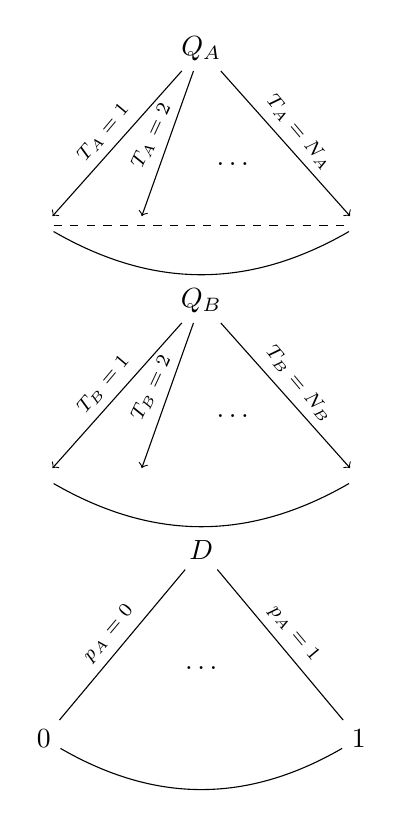
\begin{tikzpicture}[-, node distance = 2cm, scale=0.8]
    \node[anchor=north](QA){\(Q_A\)};
    \node[anchor=north](QA_d1) at (-2.5, -3) {};
    \node[anchor=north](QA_d2) at (-1, -3) {};
    \node[anchor=north](QA_d3) at (0.5, -2) {\(\dots\)};
    \node[anchor=north](QA_d4) at (2.5, -3) {};

    \path[->] (QA) edge node [above, rotate=50] {\scriptsize{\(T_A=1\)}}(QA_d1);
    \path[->] (QA) edge node [above, rotate=65] {\scriptsize{\(T_A=2\)}}(QA_d2);
    \path[<-] (QA_d4) edge node [above, rotate=310] {\scriptsize{\(T_A = N_A\)}}(QA);

    \path (QA_d1) [dashed] edge node {}(QA_d4);
    \path (QA_d1) [bend right] edge node {}(QA_d4);

    \node[anchor=north](QB) at (0, -4) {\(Q_B\)};
    \node[anchor=north](QB_d1) at (-2.5, -7) {};
    \node[anchor=north](QB_d2) at (-1, -7) {};
    \node[anchor=north](QB_d3) at (0.5, -6) {\(\dots\)};
    \node[anchor=north](QB_d4) at (2.5, -7) {};

    \path[->] (QB) edge node [above, rotate=50] {\scriptsize{\(T_B=1\)}}(QB_d1);
    \path[->] (QB) edge node [above, rotate=65] {\scriptsize{\(T_B=2\)}}(QB_d2);
    \path[<-] (QB_d4) edge node [above, rotate=310] {\scriptsize{\(T_B = N_B\)}}(QB);

    \path (QB_d1) [bend right] edge node {}(QB_d4);

    \node[anchor=north] (D) at (0, -8) {\(D\)};
    \node[anchor=north](D_d1) at (-2.5, -11) {0};
    \node[anchor=north](D_dots) at (0, -10) {\(\dots\)};
    \node[anchor=north](D_d2) at (2.5, -11) {1};

    \path[-] (D) edge node [above, rotate=50] {\scriptsize{\(p_A=0\)}}(D_d1);
    \path[-] (D_d2) edge node [above, rotate=310] {\scriptsize{\(p_A=1\)}}(D);

    \path (D_d1) [bend right] edge node {}(D_d2);

\end{tikzpicture}

    \caption{Imperfect information extensive form game between the distribution
    service and the 2 queueing systems}
    \label{fig:imperfect_info_game}
\end{figure}

The game tree is a representation of all possible sequences of decisions that
can be made by the players.
Initially, queueing system \(A\) chooses which threshold \(T_A\) to play out of
\(N_A\) possible choices.
Then, queueing system \(B\) chooses its own threshold \(Q_B\) without knowing
the threshold chosen by queueing system \(A\).
Note here that it doesn't matter which queueing system chooses its threshold
first since the other queueing system will always choose its threshold
independently of the first queueing system's choice.
Afterwards, the distribution service chooses the proportion of individuals to
send to queueing system \(A\), from the continuous strategy space of
\(0 \leq p_A \leq 1\).
The distribution service has all the information about the state that the game
is at when it's choosing the value of \(p_A\).
Thus, the distribution service's choice of \(p_A\) is based on the thresholds
chosen by the queueing systems.
The payoffs for all players are then calculated.